 
\section{Metodología}

\subsection{Obtención de datos}

El proceso de obtención de datos se lo realizó tomando imágenes satelitales que provee el satélite
Landsat 7. En este proceso se descargaron 1362 imágenes satelitales desde el año 1999 hasta el año 2015, que cubren el 
departamento de Nariño. Para cubrir todo el departamento fue necesario descargar las imagenes satelitales con 
los siguientes paths y rows: (009,059), (009,060), (010,058), (010,059), (011,059) 

En la obtención de datos también se utilizó el mapa de biomass construido por \cite{baccini2012estimated} 
construido para el año 2000 a 2003.


\subsection{Preprocesamiento}

En esta etapa de preprocesamiento se reproyecto las imágenes obtenidas, debido a que las cinco imágenes
que cubren el departamento de Nariño, estan en distintos sistemas de coordenadas (EPSG:32618 y EPSG:32617) y se 
lo reproyecto al sitema EPSG:3857. Así como también se recorto las imágenes con el fin de unicamente tener 
el área que cubre el departamento de Nariño.

\begin{figure*}
  \centering
  \subfigure[Imágenes Satélitales de Nariño]{\label{Imágenes Satélitales Nariño} 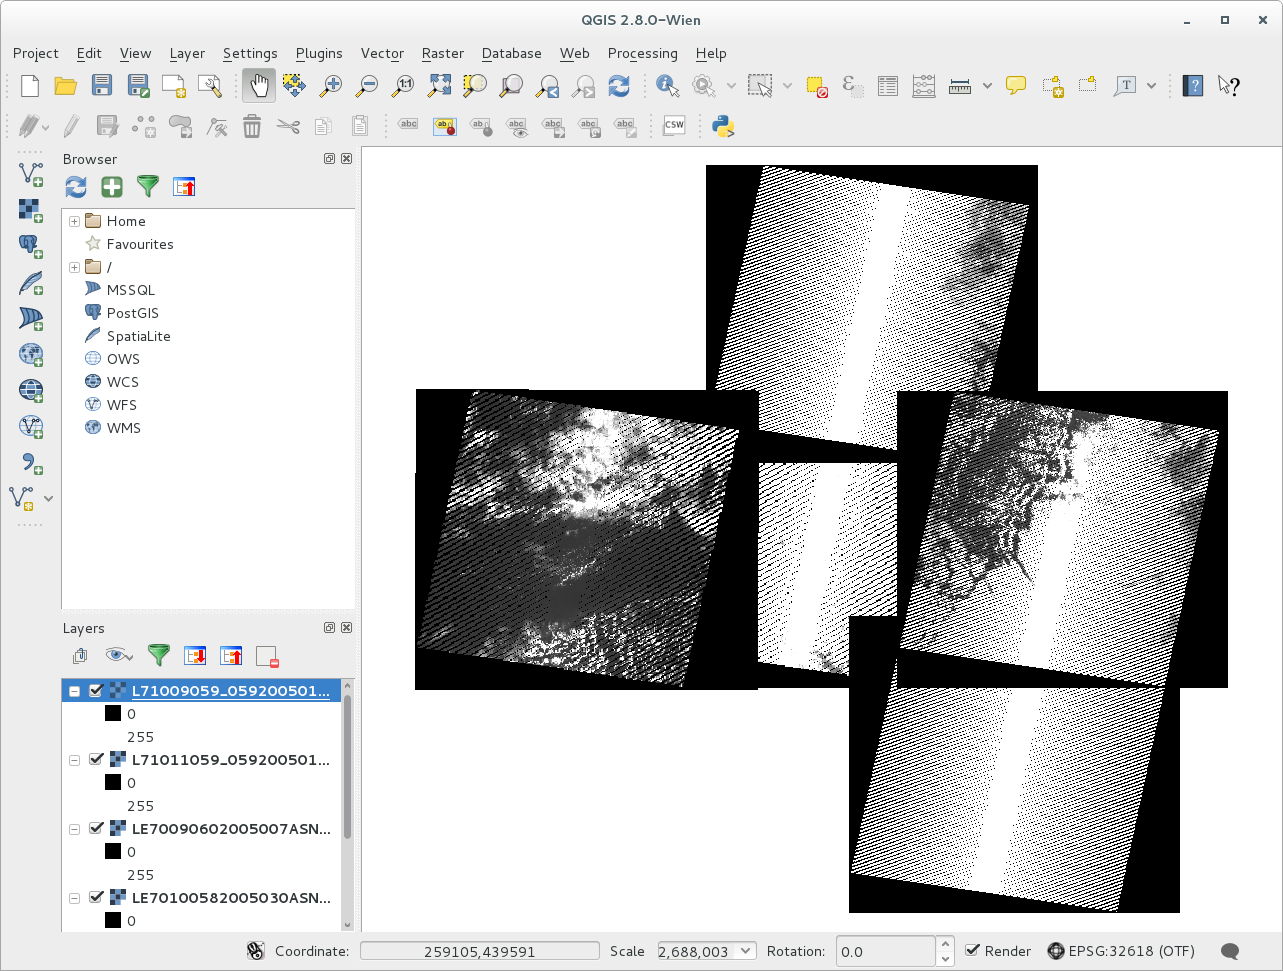
\includegraphics[width= 4cm]{cut1.png}}
  \vfill
  \subfigure[Imágenes recortadas de Nariño]{\label{Imágenes recortadas de Nariño}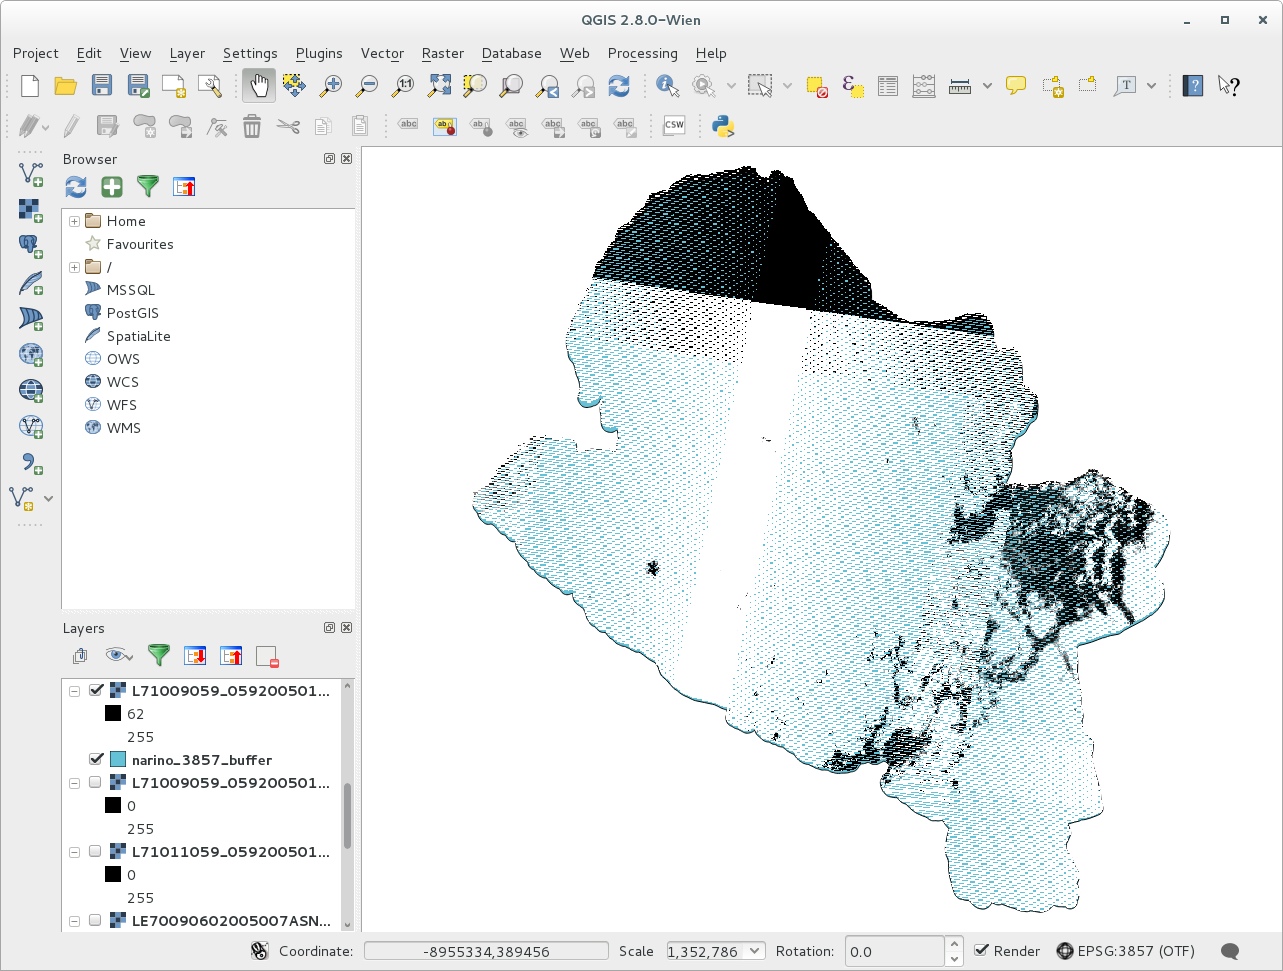
\includegraphics[width= 4cm]{cut2.png}}
  \caption{Prepocesamiento}
  \label{fig:Recortar imágenes}
\end{figure*}


De igual manera este proceso se lo realizó para el mapa de biomasa, como se muestra en la figura~\ref{fig:mapaNarino}


\begin{figure}
  \centering
  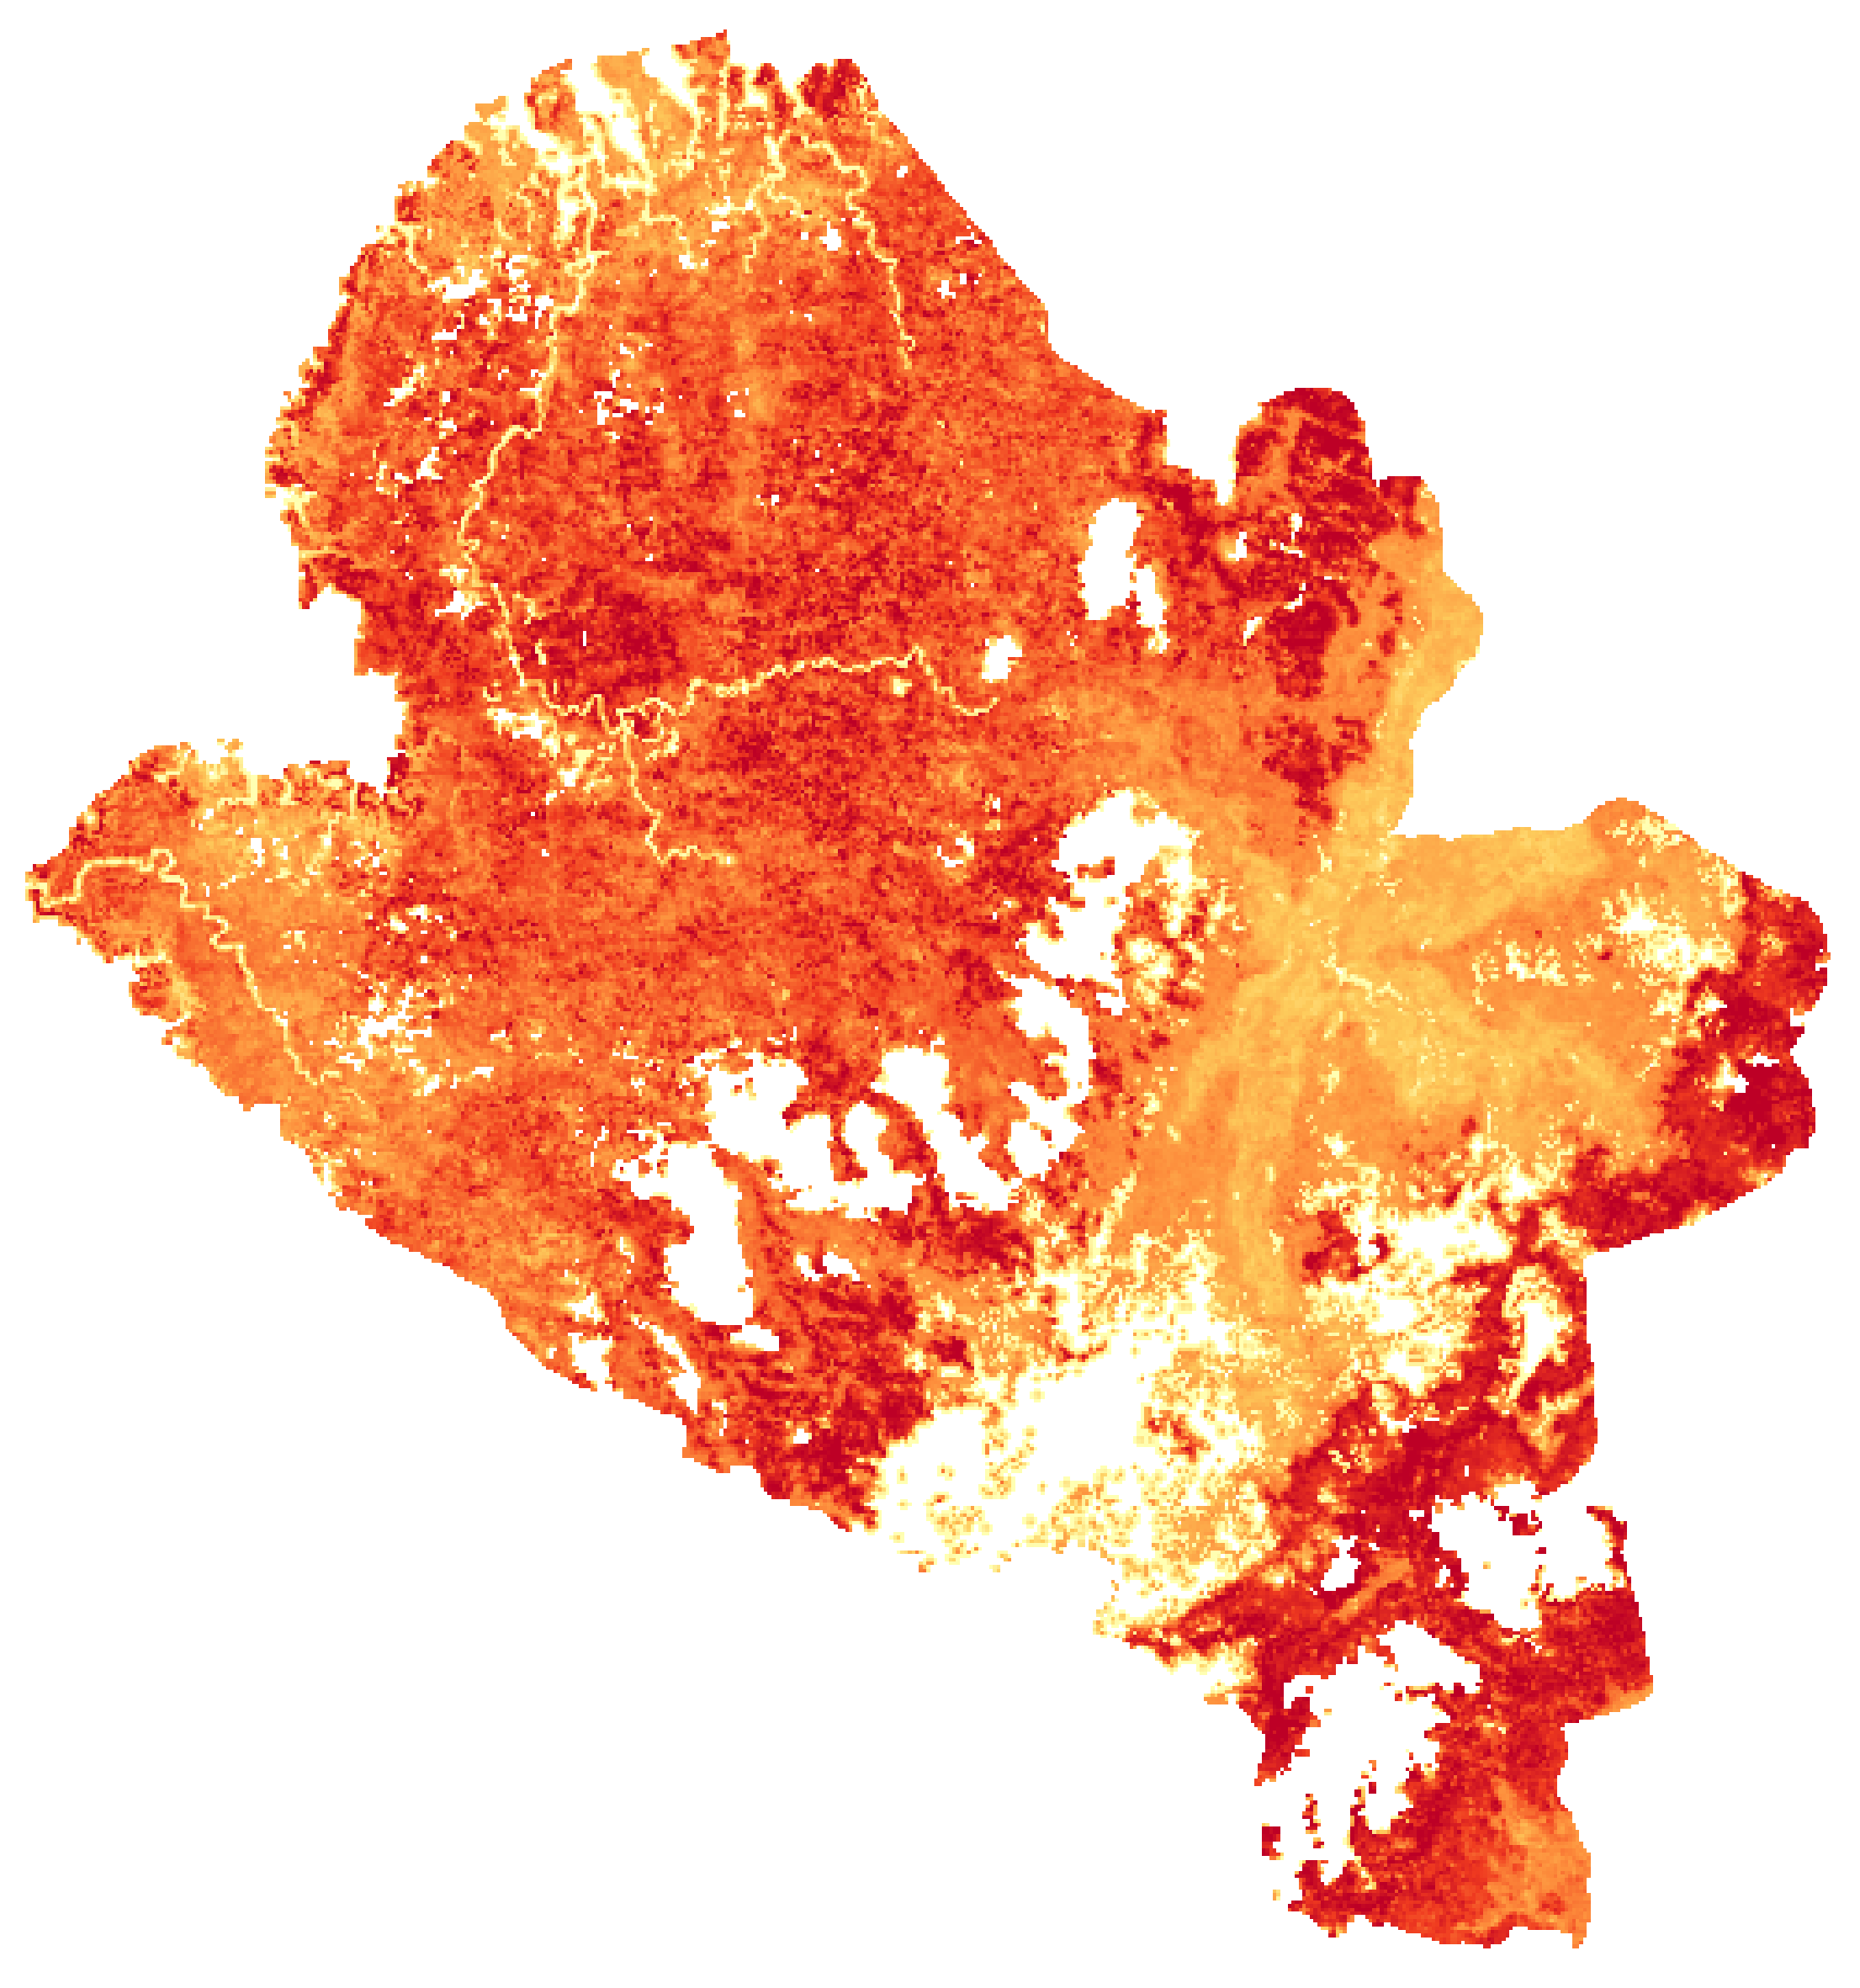
\includegraphics[width = 5cm]{mapaNarino.png}
  \caption{Mapa de Nariño .}
  \label{fig:mapaNarino}
\end{figure}

\subsection{Procesamiento y limpieza de datos}

Para esta etapa, primero se diseño una base de datos para capturar los datos,
como lo muestra la figura~\ref{fig:landsatET}, la cual tiene 4 tablas. 

Tabla date\_landsat: en la cual se almacenan las fechas de las imágenes satelitales.

Tabla reflectance: en la cual se almacenan los datos capturados y convertidos en reflentance,
de las bandas landsat (1,2,3,4,5,7) y la temperatura en grados kelvin de la banda 6.

Tabla discarded: en la cual se almacenan datos que fueron descartados, por varias rasones,
son nubes calientes, nubes frias, datos ambiguos o no son vegetación.

Tabla biomass: en la cual se almacenan los datos de biomassa del mapa de \cite{baccini2012estimated}.

Para procesar las imágenes y llenar la base de datos se realizó un Script, el cual captura el Digital Number
de las imágenes satélitales y lo transforma en valor de reflectance.

\begin{figure}
  \centering
  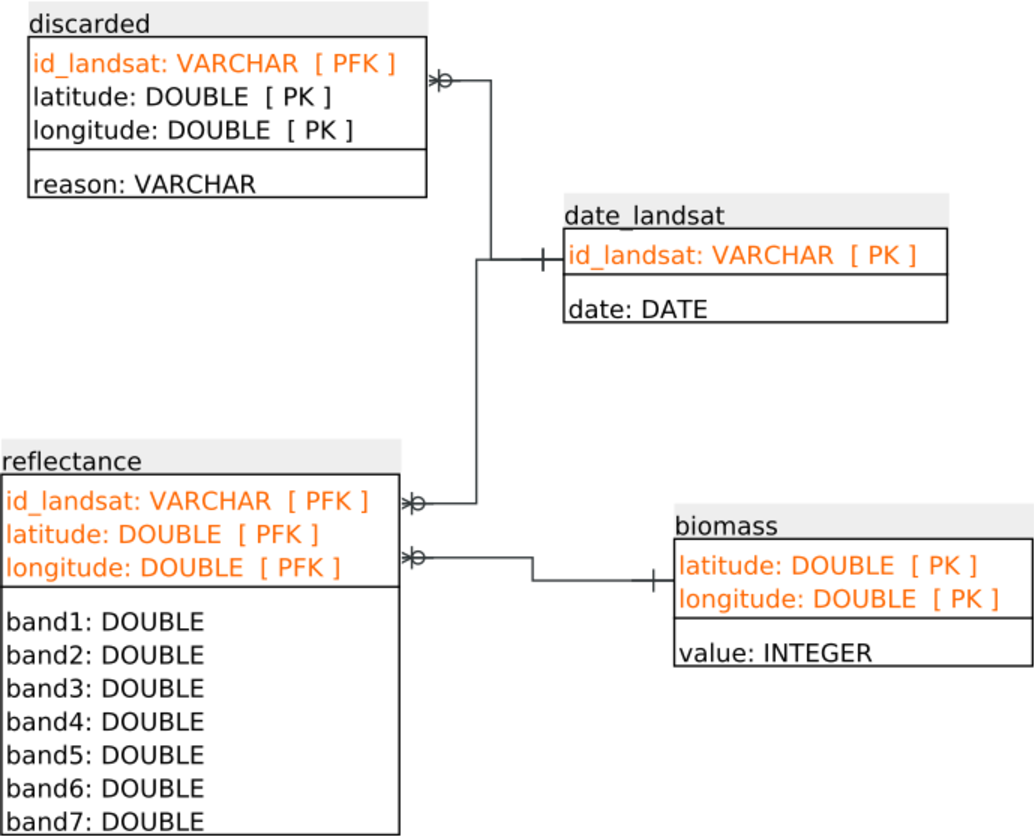
\includegraphics[width = 8cm]{landsatET.pdf}
  \caption{Modelo entidad-relacion Landsat}
  \label{fig:landsatET}
\end{figure}



